\chapter{Discussão}\label{cap:discussao}

Os dados extraídos e o conhecimento obtido pela leitura dos
artigos subsidiam as respostas para as questões de pesquisa e uma
discussão com considerações gerais da área investigada, que são apresentadas
neste capítulo.

\section{Técnicas de negociação de requisitos}

Foram encontradas 10 técnicas de negociação de requisitos, que são descritas
abaixo, a fim de responder a questão principal da pesquisa.

\begin{description}
\setlength{\itemsep}{1pt}
\setlength{\itemindent}{20pt}
\item [I \textit{WinWin}:]

O modelo \textit{WinWin} se baseia na teoria W. A técnica identificada, aqui
chamada também como \textit{WinWin} segue as etapas abaixo, valendo se de alguns
conceitos apresentados a seguir.
Condições de vitória são os objetivos ou
preocupações com o sistema, pelos \textit{stakeholders}. Quando condições de
vitória são conflitantes, se tem um ou mais problemas, que os
\textit{stakeholders} podem debater, dando opções para resolvê-lo(s). Quando uma
opção for escolhida, se firma um acordo. Este acordo por sua vez contempla de certa maneira as condições de vitória, excluindo
então os problemas.

 \begin{enumerate}
\item identificação dos \textit{stakeholders}
\item detectar condições de vitória dos \textit{stakeholders}
\item negociar a reconciliação das condições de vitória
 \end{enumerate}

Quando esta técnica é aplicada usando o modelo espiral, ela sofre uma
modificação de forma que um requisito novo possa ser inserido, esta atividade
normalmente desequilibra o estado \textit{WinWin} (ganha, ganha) dos
\textit{stakeholders}, sendo assim alguns passos são incluídos, como validar e
verificar o que foi negociado, analisar riscos para o próximo nível e, quando um
novo requisito for incluído, analisar o conflito deste com os já existentes.

\item [II \textit{Quantitative WinWin}:]

A técnica \textit{Quantitative WinWin} é bastante similar à técnica
\textit{WinWin}, porém esta nova técnica utiliza AHP (\textit{Analytic
Hierarchy Process}) para classificar os requisitos e \textit{stakeholders},
quantificando suas importâncias para o valor final agregado ao negócio do sistema a ser desenvolvido.
Os \textit{sets} de requisitos e de \textit{stakeholders} são identificados,
classificados, estimados mediante o esforço para cada requisito e, por último
é feita uma série de iterações de análise para se determinar o resultado ótimo
em termos de agrado aos \textit{stakeholders}.

\item [III MPARN:]

A técnica de \textit{Multi-Criteria Preference Analysis Requirements
Negotiation} (MPARN) tem como base o modelo \textit{WinWin} de negociação,
entretanto não se fundamenta em aspectos subjetivos e busca a sistematização por meio de uma
análise sistemática de preferências usando pesos e pontuações, a fim de definir
os critérios. A técnica MPARN segue os seguintes passos:

 \begin{enumerate}
\item identificar condições de vitória dos \textit{stakeholders}
\item identificar problemas/conflitos entre as condições de vitória
\item explorar opções de resolução de conflitos
\item explorar critérios objetivos
\item avaliar pontuação de opções baseadas em critérios
\item avaliar pesos de critérios relativos para cada \textit{stakeholder}
\item rankear opções
\item pós análise, para acordos
 \end{enumerate}

\item [IV Win CBAM:]

O Win CBAM é uma técnica de negociação que visa definir soluções quando houver a
necessidade de reconciliação, focando no custo x benefício das opções. Ele
define os seguintes passos:

 \begin{enumerate}
\item elicitar condições de vitória dos \textit{stakeholders}
\item identificar problemas de conflito entre as condições de vitória
\item explorar opções ou estratégias de arquitetura
\item avaliar os benefícios dos atributos de qualidade
\item quantificar os benefícios das estratégias arquiteturais
\item quantificar as implicações de custo e prazo das estratégias arquiteturais
\item calcular a desejabilidade
\item alcançar acordos
 \end{enumerate}

\item [V \textit{Requirement Negotiation Spiral Model}:]

Essa técnica é similar ao \textit{WinWin}, porém alguns passos possuem uma
semântica diferente e existem ainda premissas para que ele seja aplicado, portanto é de
certa forma diferente. Seus passos seguem abaixo.
 
 \begin{enumerate}
\item Identificar conflitos
\item Desenvolvimento de soluções alternativas
\item Elaboração de soluções
\item Julgamento e troca
\item Avaliar e analisar acordo entre partes
 \end{enumerate}

Para a técnica funcionar, são necessários 3 elementos externos, cenário:
critério e estratégia de resolução. O cenário consiste em um mapeamento dos
\textit{stakeholders}, o critério seria a forma como os requisitos serão
priorizados durante os conflitos, e a estratégia é um dentre vários arquétipos de resolução
de conflito.  O processo considera que os requisitos já foram elicitados
previamente.

\item [VI \textit{QA EasyWinWin}:]

O \textit{QA EasyWinWin} é uma junção das técnicas \textit{EasyWinWin}, com
técnicas de QA (\textit{quality assurance}). Dessa forma, essa técnica segue
todos os passos de \textit{Easy WinWin}, entretanto, antes, durante e após as
negociações devem ser aplicadas as técnicas de QA.

\item [VII CBSP:]

A técnica CBSP visa transformar descrições de requisitos em descrições de
decisões arquiteturais. A interpretação dos requisitos geram impactos na
arquitetura do \textit{software} e tal interpretação pode divergir de arquiteto
para arquiteto, havendo conflitos. CBSP também define procedimentos de resolução de conflitos dada diferentes interpretações dos requisitos. Os passos definidos na técnica seguem abaixo.

 \begin{enumerate}
\item seleção de requisitos do próximo nível
\item classificação arquitetural de requisitos
\item identificação e resolução de conflitos de classificação
\item refinamento arquitetural de requisitos
\item derivação de estilo arquitetural e arquitetura
 \end{enumerate}
 
\item [VIII \textit{Easy WinWin}:]

A técnica \textit{Easy WinWin} se baseia na técnica \textit{WinWin} e seu modelo
espiral, seguindo todos os passos da mesma. Seu principal diferencial é a
colaboração dos envolvidos no processo de negociação. Para isso são abordadas formas de gerar conhecimento para todos os
\textit{stakeholders}, por exemplo, com a criação de um glossário de termos, a fim de
alinhar o conhecimento dos mesmos.
 Ela necessita, ainda, que os \textit{stakeholders} priorizem as condições de
 vitória sob os aspectos da importância de negócio e da facilidade de realização. Essa
 priorização só deve ser feita se o \textit{stakeholder} tem conhecimento o
 suficiente; por exemplo, um desenvolvedor pode não ter ideia da importância de um
 determinado requisito para o negócio e, sendo assim não deve votar sob tal
 aspecto, entretanto ele pode o fazer sob outro, por exemplo, facilidade de
 realização.
Essa priorização possui 4 classificações, que são descritas abaixo.

 \begin{itemize}
\item frutos fáceis de colher (alta prioridade, baixa dificuldade de implementar)
\item importante com obstáculos (alta prioridade, alta dificuldade de implementar)
\item talvez mais tarde (baixa prioridade, baixa dificuldade de implementar)
\item esqueça-as (baixa prioridade, alta dificuldade de implementar)
 \end{itemize}

Nesse ambiente de negociação, uma situação comum é um \textit{stakeholder} ter
se esquecido de elencar alguma condição de vitória, por exemplo, sobre a
performance do \textit{software} e outro o lembrou desse tópico.

\item [IX QFD Colaborativo:]

As etapas de QFD (\textit{Quality Function Deployment}) colaborativo são as
seguintes:

 \begin{enumerate}
\item identificar \textit{stakeholders}
\item definir requisitos de \textit{stakeholders} e por a esquerda, em uma
matriz.
\item definir especificação técnica e por no topo da matriz.
\item \textit{stakeholders} colocam valores na interseção de
requisitos/especificação técnica, esse valor descreve o quanto para ele a ligação é relevante.
\item os valores são negociados até que se tenha um valor final, que atenda à
todos os \textit{stakeholders}.
 \end{enumerate}

\item [X \textit{WinWin with Scrum}:]

A técnica apresentada claramente se baseia na técnica \textit{WinWin} e sendo
assim, possui os mesmos passos, entretanto papéis são definidos e uma ordem de reuniões, tal como o uso de artefatos.
O \textit{product backlog} e \textit{sprint backlog}, são adaptados para conter
requisitos de negociação.
O PMO define os requisitos juntamente com os clientes, o negociador master
garante o bom funcionamento das reuniões e a equipe de negociação levanta pontos a serem debatidos.
As reuniões têm o mesmo funcionamento que no scrum, tal como os papéis e os
artefatos, exemplificamos as características acima para somente contextualizar.
O principal diferencial é que deve haver uma reunião de negociação para cada
\textit{Sprint}, enquanto no \textit{WinWin} as reuniões de negociação não têm
um cronograma definido, tanto quanto não têm papeis definidos.
 \end{description}
 
 \section{Ambiente, tipos de pesquisa e tipos de estudos primários}

A grande maioria das técnicas foi aplicada apenas na academia, sendo
muito usada, inclusive, como meio de melhorar o ensino de engenharia de
\textit{software}. Muitos dos estudos primários encontrados eram experimentos
com grupos de alunos de engenharia de \textit{software} realizando projetos para
a faculdade, como um sistema de biblioteca por exemplo. Logo sabe-se pouco sobre a aderência e
a aceitabilidade de tais técnicas na indústria.

Os gráficos 3.1, 3.2 e 3.3 mostram respectivamente a proporção entre academia e
indústria, entre os tipos de pesquisa e entre os tipos de estudos primários.
Dessa forma obtemos as respostas para a primeira, a segunda e a terceira
questões secundárias.
 
 \begin{figure}[h!]
 \centering
 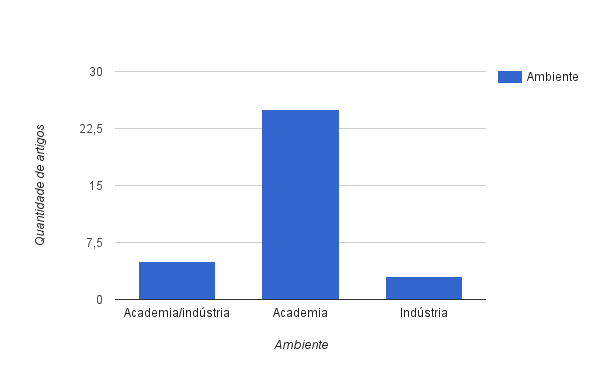
\includegraphics[scale=0.5]{tipo_de_ambiente.png}
 \caption{\label{fig:ambiente}Contagem de Artigos por Ambiente}
\end{figure}
 
 %\FloatBarrier%
 
 \begin{figure}[h!]
 \centering
 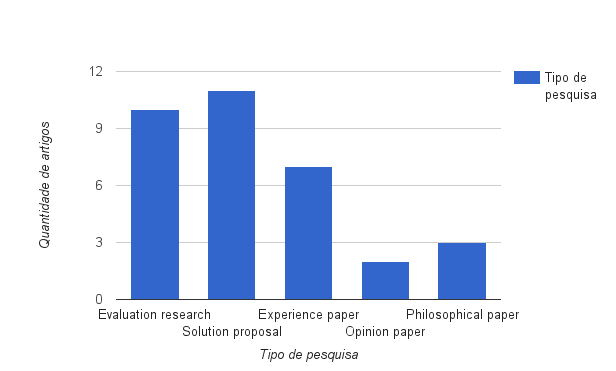
\includegraphics[scale=0.5]{tipo_de_pesquisa.png}
 \caption{\label{fig:tipo_de_pesquisa}Contagem de Artigos por Tipos de Pesquisa}
\end{figure}
 
 %\FloatBarrier%
 
 \begin{figure}[h!]
 \centering
 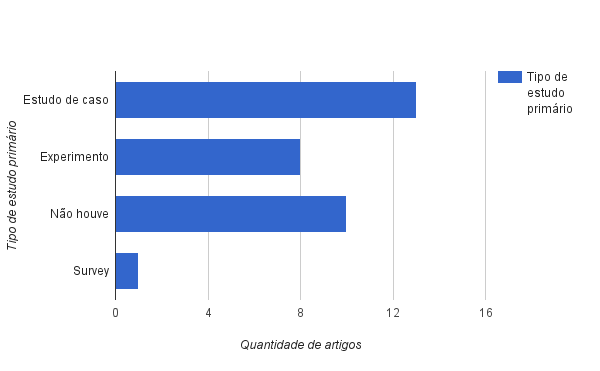
\includegraphics[scale=0.5]{tipo_de_estudo_primario.png}
 \caption{\label{fig:tipo_de_estudo_primario}Contagem de Artigos por Tipos de
 Estudos Primários}
\end{figure}
 \FloatBarrier
 
 \section{Vantagens, desvantagens e achados principais}
 
 A medida que fomos encontrando novas técnicas de negociação e catalogando suas
 vantagens, desvantagens e seus achados, era
 inevitável que fôssemos comparando as diferentes técnicas nesses quesitos.
 Algo que ficou claro, não existe uma '\textit{silver bullet}', uma técnica que
 seja ideal para qualquer tipo de projeto em qualquer organização. É possível de certa forma, dadas algumas características, escolher uma técnica que mais se enquadre à realidade dos \textit{stakeholders}. Por isso podemos seguramente
 dizer que a escolha de uma técnica é um cenário de \textit{trade-off}. O
 objetivo dessa seção é de guiar um provável usuário de técnicas de negociação
 de requisitos pelas características das mesmas auxiliando-o a descobrir qual
 a melhor opção para o seu contexto, além de responder a quarta e a quinta questões secundárias.

\subsection{Vantagens}

O \textit{WinWin}, quando aplicado usando o modelo espiral, e o \textit{WinWin
with Scrum} suportam mudanças e aceitam novos requisitos em qualquer etapa da
 negociação \cite{boehm2001developing}\cite{khan2014integration}.
O \textit{WinWin with Scrum} e o \textit{Easy WinWin} têm como vantagem um tempo
de duração menor para alcançar os objetivos
\cite{khan2014integration}\cite{briggs2002easywinwin}. Esta última e o
\textit{WinWin} abordam bem a questão de comunicação e colaboração entre os
\textit{stakeholders} \cite{grunbacher2001surfacing}\cite{boehm1998winwin}.
O \textit{Easy WinWin} chega ao ponto de tentar impedir que os
\textit{stakeholders} sejam julgados por suas opiniões
\cite{gruenbacher2000collaborative}.
O Win CBAM, o CBSP e o \textit{QA Easy WinWin} avaliam a concordância dos
\textit{stakeholders}
\cite{kazman2005requirements}\cite{grunbacher2001reconciling}\cite{grunbacher2004integrating},
sendo que estas duas últimas técnicas ainda promovem a compreensão entre
diferentes pontos de vista (técnica vs. funcional)
\cite{grunbacher2001reconciling}\cite{grunbacher2004integrating}. Enquanto a
última das mencionadas, juntamente com o \textit{WinWin}, apresentam
flexibilidade de domínio \cite{grunbacher2004integrating}\cite{boehm1997developing}, o
\textit{Quantitative WinWin} e o MPARN, diferentemente de todas as outras
técnicas, focam em adaptar o \textit{WinWin} para ter uma tomada de decisão mais
pontual e objetiva \cite{ruhe2002quantitative}\cite{in2004requirements}.


\subsection{Desvantagens}

Uma grande parte dos artigos analisados não continham estudos primários que
sustentassem achados de fato. A maioria deles, de certa forma, defendia o uso da
técnica apresentada no contexto do artigo, logo não costumavam falar diretamente
as desvantagens das técnicas. Devido a estes fatos, as desvantagens a seguir
foram resultado da nossa interpretação do material coletado de cada técnica.

No \textit{WinWin} mesmo havendo um sentimento geral de colaboração, ao final
das negociações os \textit{stakeholders} podem não se sentir completamente
satisfeitos com a especificação, porque podem, as vezes, ter cedido demais.
O \textit{WinWin} por ser bastante subjetivo \cite{ruhe2002software},pode fazer
com que sejam necessárias bem mais reuniões de negociação para analisar um set
de requisitos, do que o \textit{Easy WinWin}.
O \textit{quantitative WinWin} e MPARN são altamente dependentes de ferramentas,
visto que sendo técnicas objetivas, os \textit{stakeholders} precisam ser
guiados para não esquecer de realizar comparações. Pode-se haver perda do foco durante a tarefa
de comparação dos requisitos, caso hajam muitos a serem analisados. O MPARN ajuda para decisões locais, entretanto para decisões globais não é completamente efetivo.
\textit{Quantitative winwin}, MPARN e \textit{requeriment negotiation spiral
model} não tiveram suas vantagens comprovadas, sendo assim têm baixa
confiabilidade. \cite{ruhe2002quantitative}\cite{in2004requirements}

\subsection{Achados}

\begin{itemize}
\setlength{\itemsep}{1pt}
\setlength{\itemindent}{20pt}
\item Usuários e clientes são mais ativos em definir condições de vitória,
enquanto desenvolvedores e analistas foram mais ativos em resolver os conflitos,
tentando achar alternativas. \cite{in2001applying}
\item Existem várias formas de se aplicar o MPARN, devido a grandes quantidades
de funções para serem usadas em seus passos matemáticos. \cite{in2002multi}
\item \textit{Easy WinWin} ajuda na documentação e é interessante associá-lo a
técnica de inspeção. \cite{khan2014integration}
\item \textit{Stakeholders} tendem a aceitar condições de vitória satisfatórias
e, quando conquistadas, não se empenham com ímpeto em alcançar a solução ótima para
si. \cite{in2001applying}
\item É importante prototipar durante o desenvolvimento e negociação, para que o
usuário e cliente não mudem de ideia ao final das negociações como um todo.
\cite{boehm1998using}
\item Muitas condições de vitória podem ser alcançadas usando-se
\textit{brainstorming}.
\cite{grunbacher2001surfacing}
\item \textit{Face to face} traz sensação de segurança. \cite{egyed1997analysis}
\end{itemize} 
 
\section{Considerações Gerais da Área}

Não encontramos na literatura uma taxonomia clara e uniforme para técnicas de
negociação de requisitos. Foram encontrados, por exemplo, artigos onde
definia-se negociação como a priorização de requisitos feita apenas por um
\textit{stakeholder}. Sendo assim, não consideramos esse caso como técnica de
negociação, pois não se pode negociar consigo mesmo.

\textit{WinWin} e \textit{Spiral WinWin} são modelos de negociação de
requisitos, ou seja, são um arcabouço, cuja estrutura direciona o que deve ser alcançado. Em diversos
artigos, entretanto, eram explicitados passos que poderiam ser seguidos pelos \textit{stakeholders}. Por este motivo criamos, de certa forma, uma técnica de negociação de
requisitos chamada \textit{WinWin}.


Nos mesmos artigos onde encontramos o \textit{WinWin} e o \textit{Spiral
WinWin}, os nomes eram trocados diversas vezes, porém se referindo à um mesmo
conceito.
Como feito em \cite{boehm2006winwin}, que na introdução contextualizava o \textit{Spiral WinWin}, o qual seria a base do artigo, contudo, nas seções seguintes haviam passagens onde
falava-se do \textit{WinWin} e a imagem usada para exemplificar visualmente,
continha uma representação em espiral; outras vezes ainda no texto, tornava à aparecer
\textit{WinWin}. Dessa forma, o artigo não deixava claro se tratava de um, de
outro, ou ambos.

Eventualmente, encontrávamos artigos, cujo tema era \textit{framework}. Essa
palavra pode se referir à uma técnica ou uma ferramenta, por isso houve dificuldade de
compreensão, cabendo então interpretação.

Nossa intenção com esta revisão era encontrar uma certa variedade de técnicas de
negociação de requisitos e classificar cada uma delas, tendo como objetivo
situá-las num ambiente e contexto para permitir que \textit{stakeholders}
escolham a mais adequada, dada a conjuntura no qual eles estão inseridos. Mas o
que encontramos foi basicamente uma técnica, \textit{WinWin}, e suas diversas variações. Essas
variações abordavam diferentes focos (arquitetura, custo e etc.), bem como
diferentes formas de classificar e quantificar o valor de cada requisito.